\documentclass{article}
\usepackage{graphicx}
\usepackage{url}
\title{Prime Knots with as many as Seven Crossings}
\author{Low Dimensional Topology}

\begin{document}
\maketitle

\begin{figure}[!htb]
\minipage{0.32\textwidth}
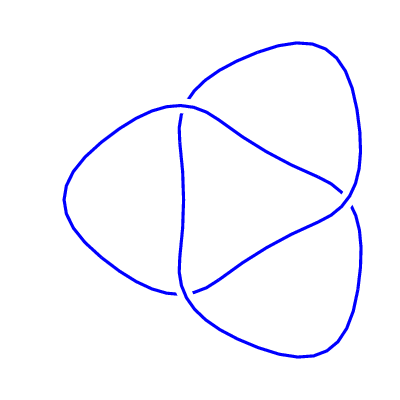
\includegraphics[width=\linewidth]{3_1.png}
\caption{Knot $3_1$, the trefoil}
\endminipage\hfill
\minipage{0.32\textwidth}
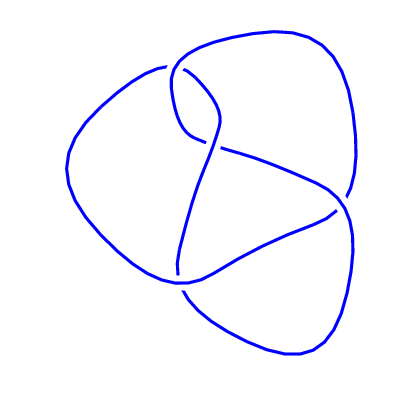
\includegraphics[width=\linewidth]{4_1.png}
\caption{Knot $4_1$, the figure eight}
\endminipage\hfill
\minipage{0.32\textwidth}
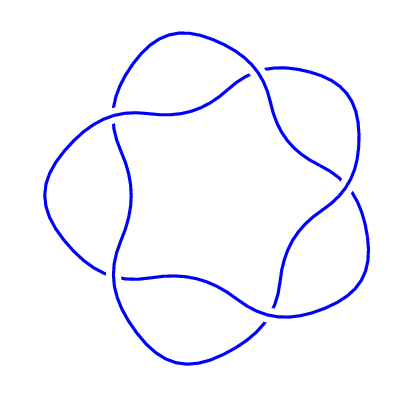
\includegraphics[width=\linewidth]{5_1.png}
\caption{Knot $5_1$}
\endminipage\hfill
\end{figure}

\begin{figure}[!htb]
\minipage{0.32\textwidth}
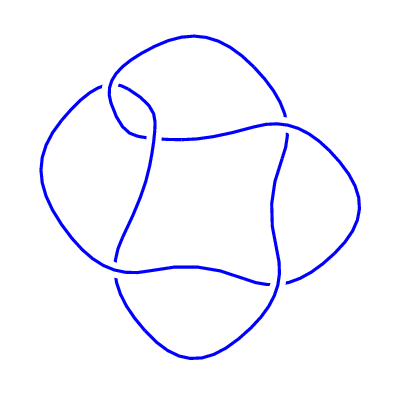
\includegraphics[width=\linewidth]{5_2.png}
\caption{Knot $5_2$}
\endminipage\hfill
\minipage{0.32\textwidth}
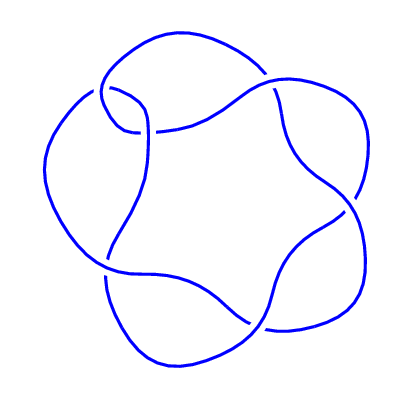
\includegraphics[width=\linewidth]{6_1.png}
\caption{Knot $6_1$}
\endminipage\hfill
\minipage{0.32\textwidth}
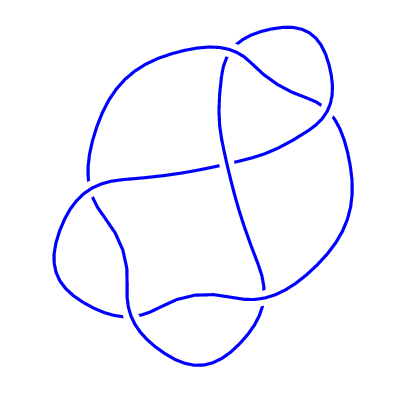
\includegraphics[width=\linewidth]{6_2.png}
\caption{Knot $6_2$}
\endminipage\hfill
\end{figure}

\begin{figure}[!htb]
\minipage{0.32\textwidth}
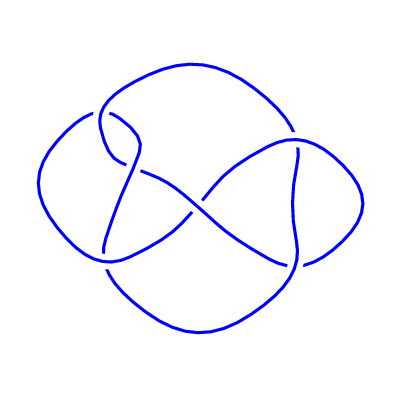
\includegraphics[width=\linewidth]{6_3.png}
\caption{Knot $6_3$}
\endminipage\hfill
\minipage{0.32\textwidth}
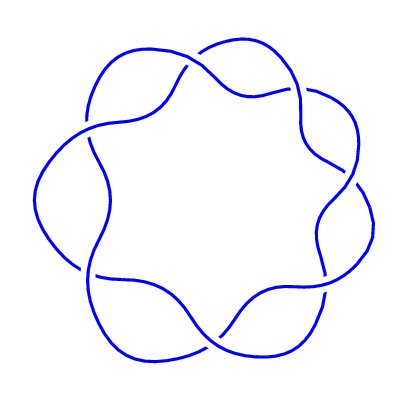
\includegraphics[width=\linewidth]{7_1.png}
\caption{Knot $7_1$}
\endminipage\hfill
\minipage{0.32\textwidth}
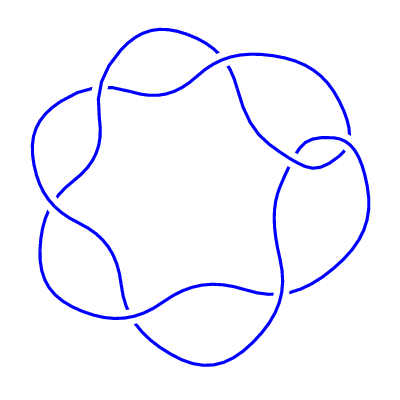
\includegraphics[width=\linewidth]{7_2.png}
\caption{Knot $7_2$}
\endminipage\hfill
\end{figure}

\begin{figure}[!htb]
\minipage{0.32\textwidth}
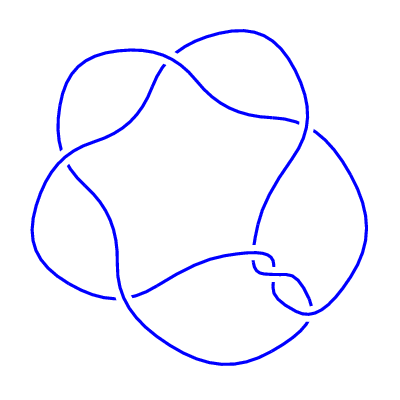
\includegraphics[width=\linewidth]{7_3.png}
\caption{Knot $7_3$}
\endminipage\hfill
\minipage{0.32\textwidth}
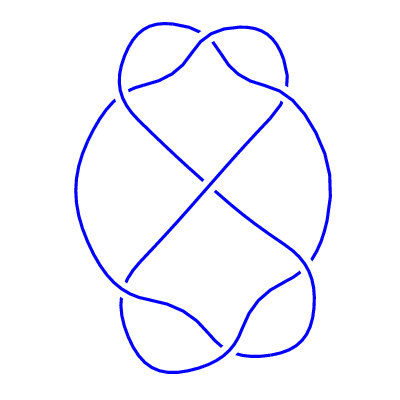
\includegraphics[width=\linewidth]{7_4.png}
\caption{Knot $7_4$}
\endminipage\hfill
\minipage{0.32\textwidth}
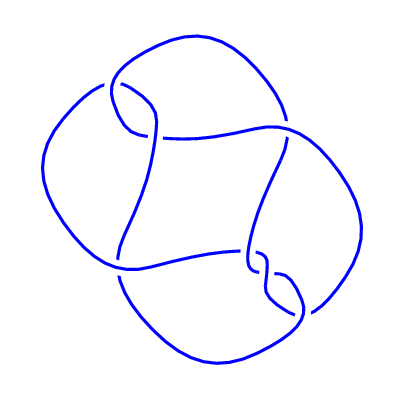
\includegraphics[width=\linewidth]{7_5.png}
\caption{Knot $7_5$}
\endminipage\hfill
\end{figure}

\begin{figure}[!htb]
\minipage{0.32\textwidth}
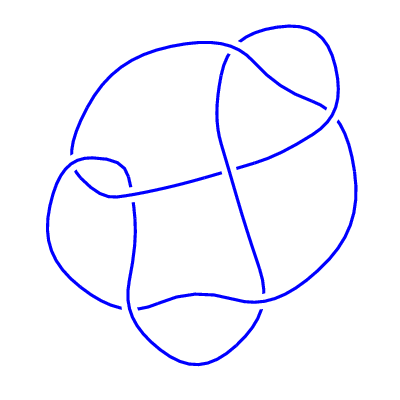
\includegraphics[width=\linewidth]{7_6.png}
\caption{Knot $7_6$}
\endminipage\hfill
\minipage{0.32\textwidth}
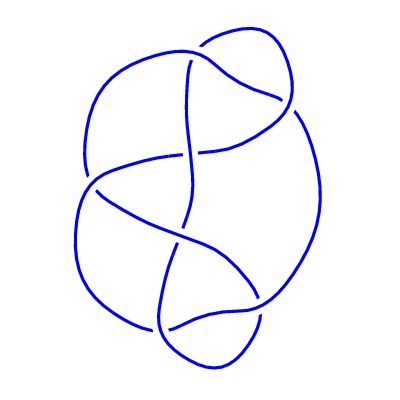
\includegraphics[width=\linewidth]{7_7.png}
\caption{Knot $7_7$}
\endminipage\hfill
\end{figure}

All of these images are taken from \url{http://www.indiana.edu/~knotinfo/}.

\end{document}
